\section{Introduction and process taxonomy}
\label{sec:intro}

\subsection{Scope and motivation}
Glass is the archetypal engineering material whose value lies in properties that most additive manufacturing (AM) routes destroy: optical transparency, chemical inertness, a smooth fire-polished surface and an amorphous, isotropic microstructure. Powder-bed sintering of glass has been demonstrated since the early 2000s, yet the parts are porous, opaque and fragile because the glass particles never fully coalesce below the liquidus \citep{klein2015,fateri2015,datsiou2021}. The decisive step for functional glass AM was therefore taken in 2014--2015 when two groups showed that glass can be deposited while it is \emph{molten}: the Mediated Matter Group at MIT built a crucible-fed extrusion printer that laid down \SI{10}{mm} cords of soda-lime glass at about \SI{1000}{\celsius} into a heated annealing chamber \citep{klein2015}, and the Kinzel group at Missouri University of Science and Technology fed a glass rod or filament into a CO$_2$-laser-generated melt pool \citep{luo2014jmse,luo2017sodalime}. Both produced optically transparent, fully dense objects directly from the melt, without debinding, sintering or post-densification.

This monograph reviews the state of the art of \emph{molten hot glass additive manufacturing} across the decade from those first demonstrations to the present (September 2026). Its scope is deliberately restricted to processes in which the glass is in a liquid or viscous-liquid state (\(\eta \lesssim 10^{6}\,\)Pa\,s) at the point of deposition or consolidation, and it treats the indirect nanocomposite routes (stereolithography, direct ink writing, thermoplastic extrusion, volumetric printing of silica-loaded polymers followed by sintering) only where a comparison is instructive. The reason for this restriction is physical rather than editorial: molten deposition is governed by the thermo-rheology of the glass melt and by the thermal history imposed on it by the machine, whereas the indirect routes are governed by colloid chemistry and by sintering kinetics of a green body. The two families share a material but not a process science.

The review was compiled autonomously from a harvested corpus. Sixty-six peer-reviewed works, four patent documents, manufacturer datasheets and industry reports were resolved through the OpenAlex and Crossref indices, open-access copies were downloaded where licences permit, and every source is listed with its digital object identifier (DOI) in the machine-readable manifest that accompanies the LaTeX source. Where a number is quoted in the text it is traceable to one of these sources; where a number is derived (for example the Vogel--Fulcher--Tammann fits in \cref{sec:physics}) the input data and the fitting procedure are stated so that the derivation can be reproduced.

\subsection{A strict taxonomy: direct versus indirect glass AM}
\Cref{fig:taxonomy} sets out the taxonomy used throughout this document. The primary split is whether the glass is molten \emph{at the moment of deposition} (direct) or is shaped cold and converted to glass by a later thermal treatment (indirect).

\begin{figure}[htbp]
  \centering
  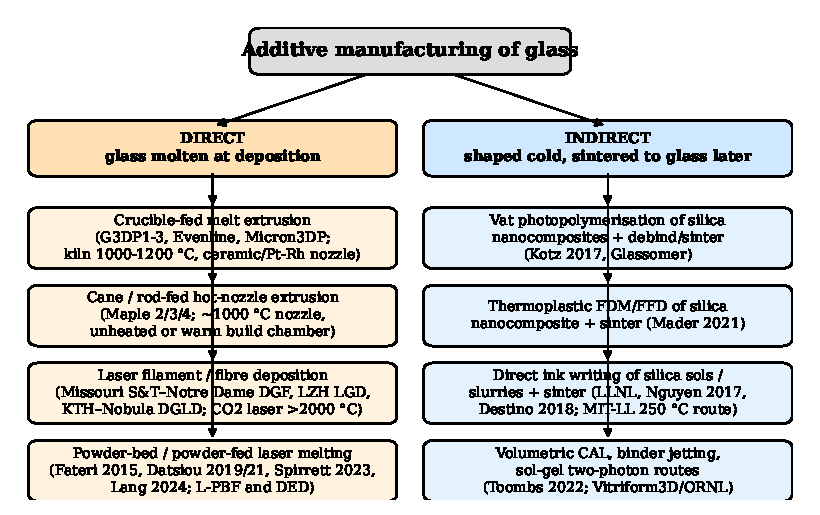
\includegraphics[width=\linewidth]{fig_taxonomy.pdf}
  \caption{Process taxonomy of glass additive manufacturing used in this review. The left branch (direct) groups processes in which the glass is in a liquid or viscous-liquid state when it is laid down or consolidated; the right branch (indirect) groups processes in which a silica-loaded polymer or sol is shaped at low temperature and converted to glass by debinding and sintering. The direct branch is the subject of this review. Representative systems and publications are named in each box; the sub-branches differ in feedstock (bulk melt, rod or cane, fibre, powder) and in heat source (resistive kiln, hot nozzle, CO$_2$ laser). Sources: \citet{klein2015,inamura2018,mit2024masonry,luo2017sodalime,witzendorff2018,kth2022bonding,fateri2015,datsiou2019,spirrett2023,lang2024,kotz2017,mader2021,nguyen2017,destino2018,toombs2022,ornl2026}.}
  \label{fig:taxonomy}
\end{figure}

Within the direct branch four sub-families are distinguished by feedstock and heat source:

\begin{enumerate}[leftmargin=*,itemsep=2pt]
  \item \textbf{Crucible-fed melt extrusion.} A charge of glass (\SIrange{2}{30}{kg}) is held molten in a refractory crucible inside an electric kiln at \SIrange{1000}{1200}{\celsius}; the melt drains under its own hydrostatic head through a heated ceramic (alumina or alumina--zirconia--silica) nozzle of \SIrange{5}{15}{mm} bore into a build chamber held near the annealing point. This is the G3DP lineage \citep{klein2015,inamura2018,mit2024masonry,patent_us10266442,patent_us9919510} and it is the only route that has produced architectural-scale parts (\SI{3}{m} columns, full-size masonry units). Deposition rates are \SIrange{2}{5}{kg/h}.
  \item \textbf{Cane- or rod-fed hot-nozzle extrusion.} A solid glass rod (``cane'') of a few millimetres diameter is pushed mechanically into a short heated nozzle at roughly \SI{1000}{\celsius} and extruded as a filament of \SIrange{0.5}{2}{mm}, analogous to polymer fused-filament fabrication. Only the last few millimetres of feedstock are molten at any time, so the thermal inertia and electrical power are small. This is the Micron3DP and Maple Glass Printing approach \citep{micron3dp_acers,maple_ammedia,threednatives2025}; the abandoned Corning application describes an induction-heated platinum--rhodium variant of the same idea \citep{patent_corning2021}.
  \item \textbf{Laser filament or fibre deposition.} A glass fibre (\SIrange{0.1}{0.2}{mm}) or rod (\SIrange{1}{3}{mm}) is fed into the focus of a CO$_2$ laser (\SI{10.6}{\micro\metre}, strongly absorbed by silicates) where it melts at \SIrange{1700}{2200}{\celsius} and wets the substrate or the previous layer. Because heating is non-contact there is no nozzle in contact with the melt and fused silica becomes printable. The process is called filament-fed or ``digital glass forming'' (DGF) by the Missouri S\&T--Notre Dame group \citep{luo2017sodalime,luo2018quartz,kinzel2025dgf}, laser glass deposition (LGD) by Laser Zentrum Hannover \citep{witzendorff2018,lgd2021coaxial,lgd2024homog}, and direct glass laser deposition (DGLD) by KTH and its spin-off Nobula \citep{kth2022bonding,kth2024microlens,nobula_web}.
  \item \textbf{Laser melting of powder (bed or blown).} Soda-lime, borosilicate or silica powder is melted track-by-track by a fibre or CO$_2$ laser either in a powder bed (L-PBF/SLM) \citep{fateri2015,khmyrov2016,datsiou2019,datsiou2021,slmirregular2023,boro2025laser} or blown coaxially into a melt pool (powder-fed directed energy deposition, DED) \citep{spirrett2023,lang2024}. The glass is molten locally, so the process belongs to the direct branch, but the short melt lifetime and the entrapped inter-particle gas leave porosity of the order of \SIrange{5}{12}{\percent} and opaque parts unless a very high energy input is used.
\end{enumerate}

A hybrid fifth category, \textbf{paste extrusion with in-situ laser melting}, deposits a water-based silica paste and immediately fuses it with a CO$_2$ laser, obtaining transparent fused silica without a furnace step \citep{ieee2019dlm,paste2024}. It is treated together with powder-fed DED.

\subsection{Why molten deposition is hard: the three couplings}
The difficulty of the direct route can be stated in one sentence: the same temperature field that must keep the glass fluid enough to flow and bond must also be steep enough to freeze the deposited cord before it slumps, and shallow enough at the end of the build to avoid thermal stress. Three couplings follow.

\emph{Rheology--geometry coupling.} The viscosity of a silicate melt changes by a decade for every \SIrange{40}{80}{\celsius} in the working range (\cref{sec:physics}). A nozzle-exit temperature of \SI{990}{\celsius} in G3DP corresponds to \(\eta \approx 640\,\)Pa\,s \citep{klein2015}; a \SI{350}{\celsius} drop across the five most recent layers, measured by infrared thermography, raises the viscosity by five orders of magnitude and is what stabilises the wall against its own weight \citep{klein2015}. Any drift in nozzle temperature therefore changes bead width, slump and layer bonding simultaneously.

\emph{Thermal--mechanical coupling.} Glass has no ductility. A temperature difference across a wall that exceeds roughly \SI{100}{\celsius} during cooling through the transformation range produces residual tensile stress that fractures the part on cooling or later in service. Molten deposition thus either requires a build chamber held near the annealing point (G3DP, \SIrange{480}{525}{\celsius}) or a heated build plate and post-anneal (laser processes, \SIrange{250}{600}{\celsius}) \citep{klein2015,inamura2018,luo2017sodalime,datsiou2019}.

\emph{Chemistry--hardware coupling.} Molten glass is a universal solvent for oxides. Every wetted component---crucible, nozzle, thermocouple sheath, build plate---is corroded, and the corrosion rate roughly doubles for each \SI{50}{\celsius} \citep{zircorr2025,pgm2010}. This is why crucible-fed machines are limited to soda-lime and (with difficulty) borosilicate glasses below \SI{1200}{\celsius}, why the Corning application specified an 80/20 platinum--rhodium nozzle \citep{patent_corning2021}, and why the fused-silica processes all use non-contact laser heating.

\subsection{Historical arc 2014--2026}
\Cref{fig:timeline} places the principal milestones on a common axis. The first period (2014--2018) was one of demonstration: automated melt extrusion at MIT (G3DP, 2015; G3DP2 with \SI{25}{kg} reservoir and four-axis bed, 2017--2018), CO$_2$-laser rod and fibre feeding at Missouri S\&T (2014--2018), quartz-fibre laser deposition at Hannover (2018), and the first commercial announcements by Micron3DP (Israel, 2015--2017). The second period (2019--2022) added the powder-bed and blown-powder variants in commercial L-PBF machines at Nottingham, systematic process-window studies of laser filament printing at KTH, and the emergence of desktop cane-fed machines from Maple Glass Printing (Melbourne, first machines 2022). The third period (2023--2026) is characterised by industrial translation and control: Evenline's third-generation G3DP3 with infrared monitoring and \SI{1200}{\celsius} capability printing recycled container and float glass and full-size interlocking masonry \citep{stern2024cgc,mit2024masonry}, Nobula's DGLD desktop printer reaching \SI{2200}{\celsius} \citep{nobula_aniwaa}, real-time thermal-camera closed-loop control of laser power in digital glass forming \citep{dgf2026control,lgd2025tempctrl}, and surface finishes of \SI{21}{nm} \(R_a\) on as-printed fused silica \citep{lgd2024homog}.

\begin{figure}[htbp]
  \centering
  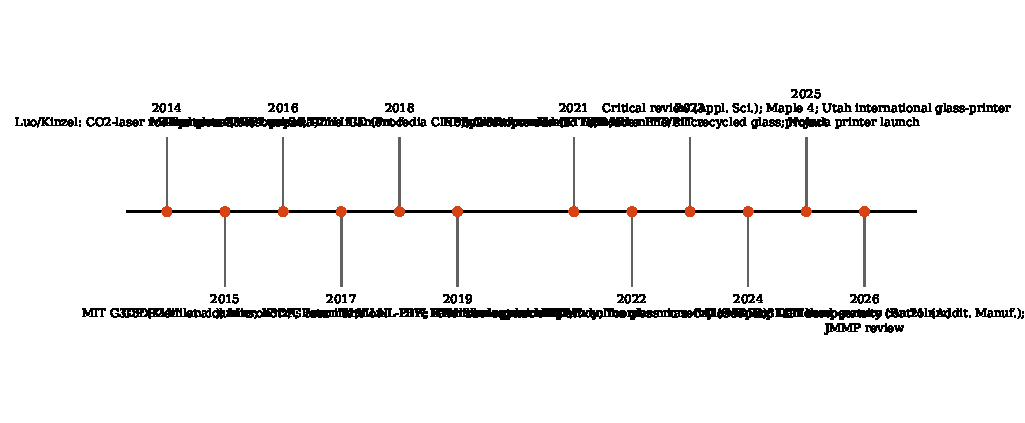
\includegraphics[width=\linewidth]{fig_timeline.pdf}
  \caption{Milestones of molten-glass additive manufacturing, 2014--2026, drawn from the harvested corpus. Events above the axis are academic, below the axis predominantly commercial or applied. Only first reports and first public machine releases are shown; incremental papers are cited in the relevant sections.}
  \label{fig:timeline}
\end{figure}

\subsection{Structure of the review}
\Cref{sec:physics} treats the materials physics: viscosity--temperature relations of the four glass families used, capillary and viscous-thread instabilities of the extruded cord, and transient heat transfer. \Cref{sec:hardware} reviews hardware: crucibles, nozzles and their materials, kiln architectures, laser heads, feed mechanisms and kinematics, and gives the modality comparison matrix (\cref{tab:modalities}). \Cref{sec:monitoring} covers in-situ thermal management, monitoring and annealing. \Cref{sec:open} formulates the open problems as explicit problem statements. \Cref{sec:academic,sec:industry} map the academic and industrial landscapes with the two directory tables, and \cref{sec:outlook} closes with a roadmap.
